\documentclass[12pt]{article}
\usepackage{geometry}
\usepackage{graphicx}
\usepackage{pdfpages}
\usepackage[utf8]{inputenc}
\geometry{lmargin=2cm,rmargin=1cm,tmargin=2cm,bmargin=2cm}
\renewcommand{\baselinestretch}{1.5} 

\begin{document}
\pagenumbering{gobble}

\begin{center}
	
\includegraphics[scale=0.5]{img_title_amsi} 
\end{center} 
\ \\
\begin{flushright}
	\textbf{{\fontsize{14}{10}\selectfont Discipline: Network programming}}
\end{flushright}
\ \\
\ \\
\ \\

\begin{center}
	\textbf{{\fontsize{15}{10}\selectfont Laboratory Work nr.5 \\
	\underline{Topic:} TCP.}}
\end{center}
\ \\
\ \\
\ \\
\ \\
\ \\
\begin{flushright}
	{\fontsize{12}{10}\selectfont 
		\textbf{Done by student:}  \rule{2cm}{0.4pt}(Untilov Andrei, gr.FAF-151) \\
		\ \\
		\ \\
		\textbf{Verified by:}      \rule{2cm}{0.4pt}(Gavrișco Alexandru)
		
		}
\end{flushright}
\vfill

\begin{center}
	\textbf{Chisinau 2018}
\end{center}

\newpage
\pagenumbering{arabic}
\setcounter{page}{2}
	\tableofcontents
	\newpage
	
	\section{Topic}
	TCP
	\section{Tasks}
\textbf{	Develop a client-server application with the following specs:}
	\begin{enumerate}
		\item Client should connect to server and allow to send commands:
		\begin{enumerate}
			\item Commands have to be inserted from keyboard;
			\item The response have to be shown to user;
		\end{enumerate}
		\item Server accepts conection from client through a port;
		\item Server gets commands from client;
		\item Server sends response to client.
	\end{enumerate}
	
	
	\textbf{Message's format:}
	\begin{enumerate}
		\item Commands must start with "/";
		\item If command accepts parameters, then parameters must be separated by " " (space).
		\item If server recieves an invalid command, it must respond an informative message.
		\item If server gets an invalid command , but there is a similar command , it has to return an informative message.
	\end{enumerate}
	

	

	\newpage
	\section{Theory}
	
	Transmission Control Protocol/Internet Protocol is a suite of communication protocols used to interconnect network devices on the internet. TCP/IP can also be used as a communications protocol in a private network (an intranet or an extranet).
	
	TCP/IP specifies how data is exchanged over the internet by providing end-to-end communications that identify how it should be broken into packets, addressed, transmitted, routed and received at the destination. TCP/IP requires little central management, and it is designed to make networks reliable, with the ability to recover automatically from the failure of any device on the network.
	
	\textbf{TCP} defines how applications can create channels of communication across a network. It also manages how a message is assembled into smaller packets before they are then transmitted over the internet and reassembled in the right order at the destination address.
	
	\textbf{IP} defines how to address and route each packet to make sure it reaches the right destination. Each gateway computer on the network checks this IP address to determine where to forward the message.
	
	
	
	
	
	
	
	
	\newpage
	\section{Task Implementation}
	
	TCP/IP uses the client/server model of communication in which a user or machine (a client) is provided a service (like sending a webpage) by another computer (a server) in the network. That's why are needed two classes Server.class and Client.class . The connection between client and server is released by socket , which specifies the connection port. 
	Both , the client and server has an object of type Socket with the same port, where client's socket connects to localhost (Figure 1.), while server's socket connects to ServerSocket.(Figure 2.)
	\begin{center}
		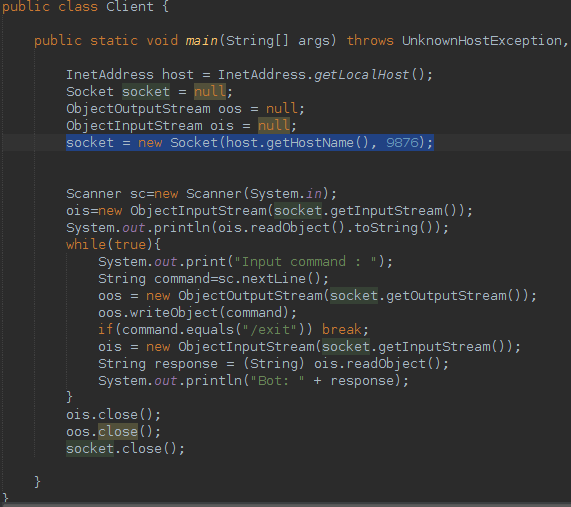
\includegraphics[scale=0.6]{clientSocket}
		
		Figure 1. - Client.java
	\end{center}
	\begin{center}
		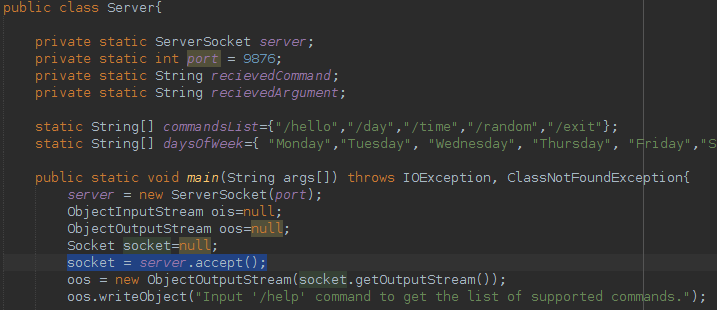
\includegraphics[scale=0.6]{serverSocket}
		
		Figure 2. - Server.java
	\end{center}
	
	The communication between server and client is performed using ObjectInputStream.java (reading data) and ObjectOutputStream.java (writing data) classes.  When client writes data to server using ObjectOutputStream, server reads data using ObjectInputStream and vice-versa.
	
	
	\begin{center}
		\textbf{*The link to repository : https://github.com/untilovandrei/PR\_Lab\_4.git}
	\end{center}
	
	
	\newpage
	\section{Conclusion}
	During this laboratory work has been obtained basic experience of working with TCP/IP protocol. It gives us the opportunity to build a flexible architecture . Also the property of  connections to remain intact as long as the source and destination machines are functioning.
	
	
	
	
\end{document}
